\section*{Chapter 14: Attention}
%\section*{Probabilities}
%\subsection*{Expect, Var, Cov, Bay}
%$\E[X]=\int_{\Omega}xf(x)\di x=\int_{\omega}x\Prob[X{=}x]\di x$ \\
\subsection*{Gating function}
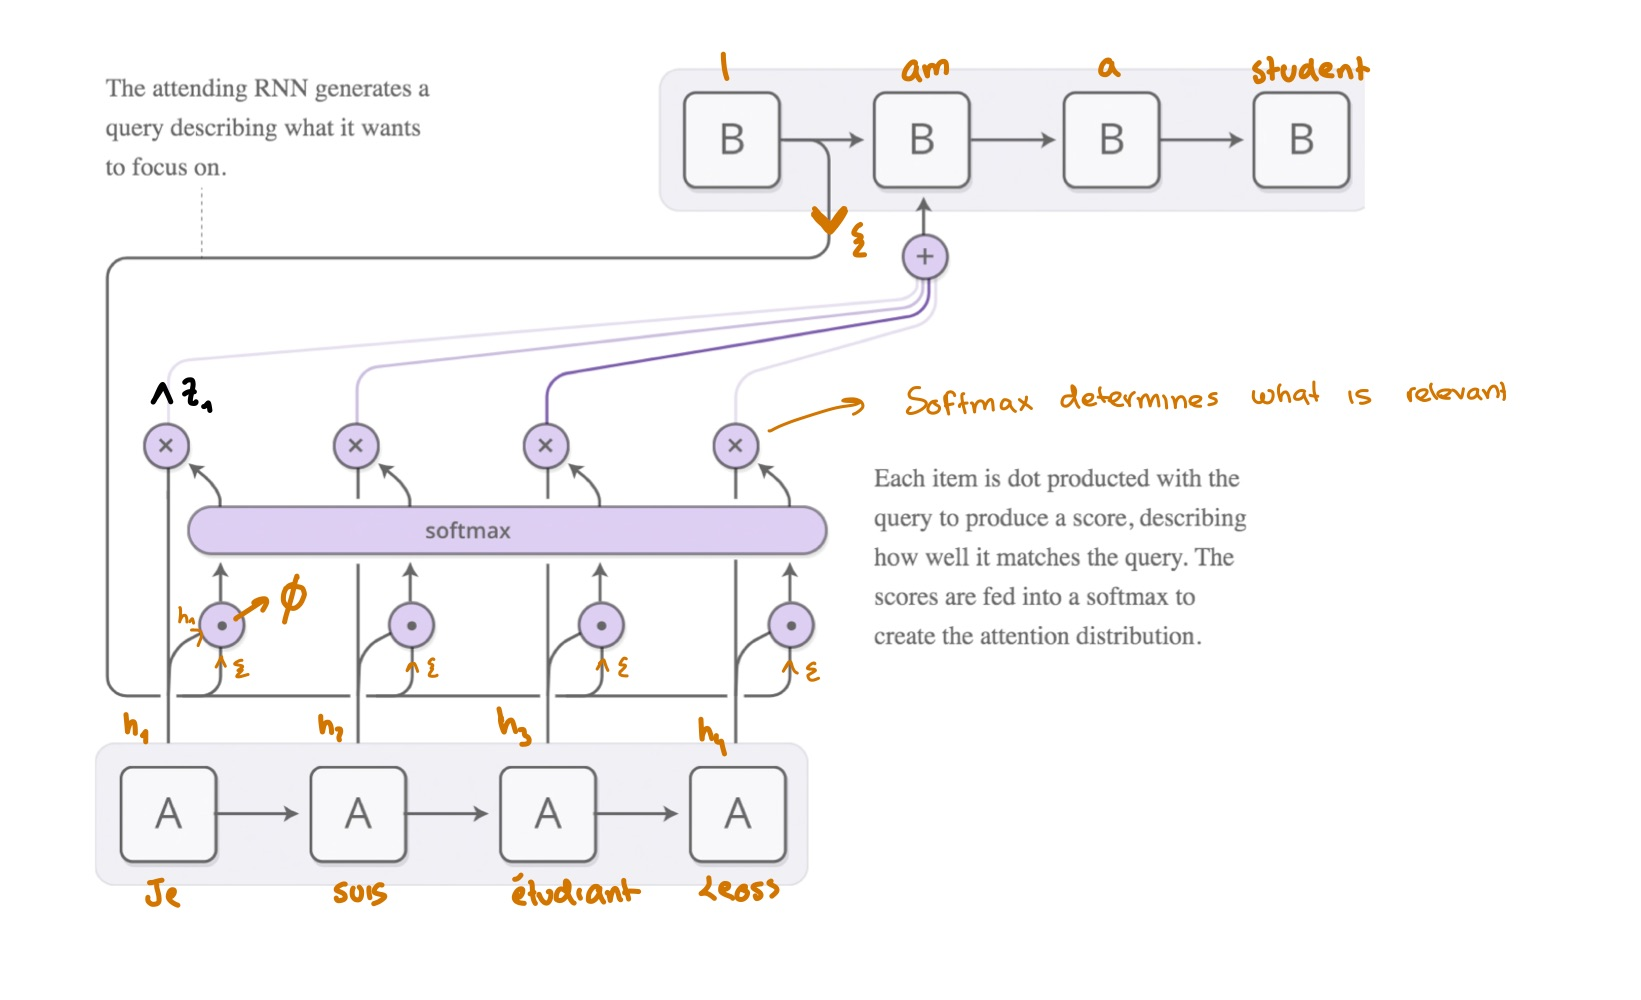
\includegraphics[width=\columnwidth]{src/gating-function.jpg}
Used in combination with RNNs to focus on relevant parts of the input depending on the desired output. Given all hidden states from the encoder ($h_e^1, ..., h_e^s$), the decoder defines a query vector $\xi \in \R^n$. Then, a function is applied between each hidden state and the query vector (can be their dot product) and a softmax on these outputs creates the attention distribution. Finally, probabilities are multiplied by their corresponding $h_e$ producing "read-outs" ($z_1, ..., z_t$) that are used as input to the decoder $(h_d^r, z^r) \mapsto y_d^{r+1}$.

\subsection*{Transformers}
Attention is all you need. Remove RNNs for efficiency. They use a stack of encoders and decoders. Each encoder is (self-attention layer + feed forward NN). Each decoder is (self-attention layer + encoder-decoder attention + feed forward NN).

\subsection*{ELMO: Contextualized Word Embeddings}
Construct embeddings that reflect context. A CNN takes as input the embedding of each input character and creates a representation for each word. Then, a bi-directional LSTM modify the representation of each word based on the context and at the end, a linear combination of all hidden layers yields the ELMO representation. Unsupervised training: predict next word.